\section{Architecture}

\begin{figure*}[ht]
\centering
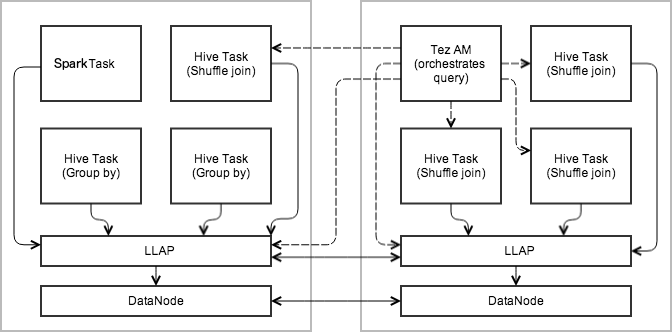
\includegraphics[width=0.8\textwidth]{figures/arch1.png}
\caption{LLAP: as an accelerator}
\label{fig:arch1}
\end{figure*} 


\emph{LLAP}, as the name suggests is a long running collection of persistent daemons, which by virtue of being always-on side-steps the
overheads of interacting with a large scale resource manager such as YARN\cite{YARN} while executing very short running queries. 

LLAP is not a SQL execution engine and neither is it a standardized store for data, but exists as an accelerated access layer with awareness of the relational
model behind the files laid out on a distributed filesystem such as HDFS, dealing with data as column \& row-groups instead of treating it as offsets. LLAP will work
within existing, process-based Hive execution to preserve the scalability and versatility of Hive.  It will not replace the existing execution model but enhances it.

The LLAP daemons are distributed across the cluster, with the service locations published to a dynamic service registry. The service registry is consumed by the 
Hive interface into LLAP, which interacts with the Tez DAG scheduler to push qualified query fragments to these service locations. The query fragments are self-contained
and are accompanied by a signed token issued at the perimeter, which forms the access control into the service. The fragment qualifications for a specific node are
primarily related to data locality, but unlike a pure-MPP system still allows for executing fragments on remote data. 

The independence of query fragments from the DAG scheduler, introduces the possibility of using a different DAG scheduler such as Apache Spark
to consume data from LLAP. The Hybrid execution model highlighted in Figure~\ref{fig:arch1}, in its simplest form 
converts LLAP into a tabular data reader service replacing direct interactions with the networked filesystem. While short running queries
can be run within LLAP entirely, the relational model offered by this interface into data is preferred over the file centric model which
can offer no security beyond file permissions. This change of roles allows for a process boundary between the user code executing within the 
hybrid tasks and allow LLAP to act as data gate for columnar access control, column masking and cell level security.

The long running nature of LLAP dove-tailed into the continued evolution of Hive's execution architecture to take advantage of the lifetime of the JVM. The multi-hour 
lifetime of the JVM allows the JDK Hotspot profiling optimizer to collect enough runtime information
to compile the core vectorized loops into \emph{SIMD} native code. To feed this CPU efficient operator pipeline, the data fetching from the storage layer
had to be revamped to buffer into temporary buffer pools so that the operator pipeline is never starved by the vagaries of the networked file
system layer. Since several processing queries share the same data sets, it is incredibly wasteful to discard buffer pools after execution which
naturally led into a cache model which can keep the uncompressed buffers in memory. And with increasing concurrency of such queries, it becomes valuable
to queue requests which have a possible cache hit in the near future instead of delegating that task to another machine without a loaded cache. To protect
latency with that the queue mechanism has to re-order internally and possibly pre-empt running tasks to avoid deadlocks. 

In following sections, we discuss the architectural components in detail.
